\documentclass[12pt]{article}
\usepackage{graphicx}
\usepackage{setspace}
\textwidth=7in
\textheight=9.5in
\topmargin=-1in
\headheight=0in
\headsep=.5in
\hoffset  -.85in

\pagestyle{empty}

\begin{document}
\doublespacing
\section{Introduction}
The Simultaneous Localisation and Mapping (SLAM) problem asks if it is possible for a mobile robot to be placed at an unknown location in an unknown environment and for the robot to incrementally build a consistent map of this environment while simultaneously determining its lo- cation within this map. A solution to the SLAM problem has been seen as a ‘holy grail’ for the mobile robotics community as it would provide the means to make a robot truly autonomous. The solution of the SLAM problem has been one of
the notable successes of the robotics community over the past decade. SLAM has been formulated and solved as a theoretical problem in a number of different forms. SLAM has also been implemented in a number of different domains from indoor robots, to outdoor, underwater and airborne systems. At a theoretical and conceptual level, SLAM can now be considered a solved problem. However, substantial issues remain in practically realizing more general SLAM solutions and notably in building and using perceptually rich maps as part of a SLAM algorithm.
\subsection{History of the SLAM Problem}

The genesis of the probabilistic SLAM problem occurred
at the 1986 IEEE Robotics and Automation Conference held in San Francisco. This was a time when probabilis- tic methods were only just beginning to be introduced into both robotics and AI. A number of researchers had been looking at applying estimation-theoretic methods to mapping and localisation problems; these included Peter Cheeseman, Jim Crowley, and Hugh Durrant-Whyte. Over the course of the conference many paper table cloths and napkins were filled with long discussions about consistent mapping. Along the way, Raja Chatila, Oliver Faugeras, Randal Smith and others also made useful contributions to the conversation.
\par The result of this conversation was a recognition that consistent probabilistic mapping was a fundamental prob- lem in robotics with major conceptual and computational issues that needed to be addressed. Over the next few years a number of key papers were produced. Work by Smith and Cheesman  and Durrant-Whyte  established a statistical basis for describing relationships between land- marks and manipulating geometric uncertainty. A key el- ement of this work was to show that there must be a high degree of correlation between estimates of the location of different landmarks in a map and that indeed these corre- lations would grow with successive observations.
\par At the same time Ayache and Faugeras  were undertaking early work in visual navigation, Crowley  and Chatila and Laumond  in sonar based navigation of mobile robots using Kalman filter-type algorithms. These two strands of research had much in common and resulted soon after in the landmark paper by Smith, Self and Cheese- man . This paper showed that as a mobile robot moves through an unknown environment taking relative observa- tions of landmarks, the estimates of these landmarks are all necessarily correlated with each other because of the common error in estimated vehicle location . The im- plication of this was profound: A consistent full solution to the combined localisation and mapping problem would require a joint state composed of the vehicle pose and every landmark position, to be updated following each landmark observation. In turn, this would require the estimator to employ a huge state vector (of order the number of land- marks maintained in the map) with computation scaling as the square of the number of landmarks.
 Crucially, this work did not look at the convergence properties of the map or its steady-state behavior. Indeed, it was widely assumed at the time that the estimated map errors would not converge and would instead exhibit a ran- dom walk behavior with unbounded error growth. Thus, given the computational complexity of the mapping prob- lem and without knowledge of the convergence behavior of the map, researchers instead focused on a series of approxi- mations to the consistent mapping problem solution which assumed or even forced the correlations between landmarks to be minimized or eliminated so reducing the full filter to a series of decoupled landmark to vehicle filters Also for these reasons, theoretical work on the combined localisation and mapping problem came to a temporary halt, with work often focused on either mapping or localisation as separate problems.
\section{Formulation and Structure of the SLAM problem}
SLAM is a process by which a mobile robot can build
a map of an environment and at the same time use this map to deduce it’s location. In SLAM both the trajectory of the platform and the location of all landmarks are esti- mated on-line without the need for any a priori knowledge of location.
A.
\begin{figure}[ht]
    \centering
    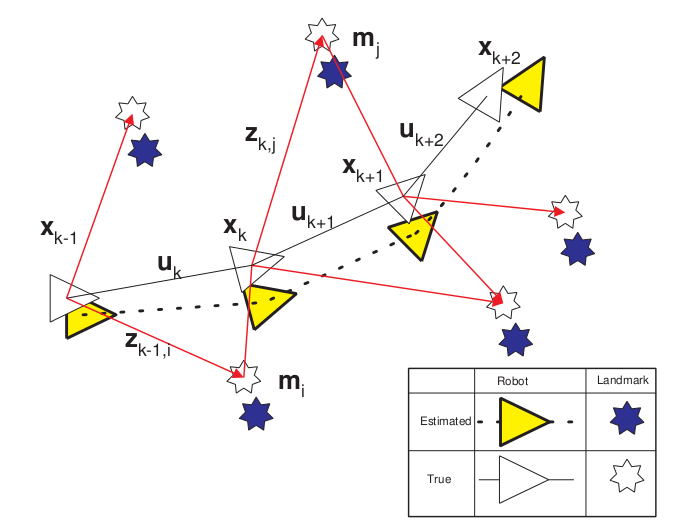
\includegraphics[width=160mm]{structure.jpg}
    \caption{The essential SLAM problem.}
    \label{slamstruct}
\end{figure} Consider a mobile robot moving through an environment
taking relative observations of a number of unknown landmarks using a sensor located on the robot as shown in Figure \ref{slamstruct}. At a time instant k, the following quantities are defined:
\begin{itemize}
\item $x_k$: The state vector describing the location and orientation of the vehicle.
\item $u_k$: The control vector, applied at time $k-1$ to drive the vehicle to a state $x_k$ at time $k$.
\item $m_i$: A vector describing the location of the $i_{th}$ landmark whose true location is assumed time invariant.
\item $z_{ik}$ : An observation taken from the vehicle of the location of the ith landmark at time $k$. When there are multiple
landmark observations at any one time or when the specific landmark is not relevant to the discussion, the observation
will be written simply as $z_k$ .\\
In addition, the following sets are also defined:
\item $X_{0:k} = {x_0,x_1,\dots,x_k} = {X_{0:k-1},x_k}$ : The history of vehicle locations.
\item $U_{0:k} = {u_1,u_2,\dots,u_k} = {U_{0:k-1},u_k}$ : The history of control inputs.
\item $m= {m_1,m_2, \dots ,m_n}$ The set of all landmarks. $Z_{0:k} = {z_1, z_2,\dots,z_k} = {Z_{0:k−1}, z_k}$ : The set of all landmark observations.
\end{itemize}
\subsection{Probabilistic SLAM}
In probabilistic form, the Simultaneous Localisation and Map Building (SLAM) problem requires that the probability distribution.
\begin{equation}
P(x_k,m|Z_{0:k},U_{0:k},x_0)
\end{equation}
be computed for all times $k$. This probability distribution describes the joint posterior density of the landmark locations and vehicle state (at time k) given the recorded observations and control inputs up to and including time k together with the initial state of the vehicle. In general, a recursive solution to the SLAM problem is desirable. Starting with an estimate for the distribution
$P(x_{k−1},m| Z_{0:k−1},U_{0:k−1})$ at time $k-1$, the joint posterior, following a control $u_k$ and observation $z_k$, is computed using Bayes Theorem. This computation requires that a state transition model and an observation model are defined describing the effect of the control input and observation respectively.
\par The observation model describes the probability of making an observation zk when the vehicle location and landmark locations are known, and is generally described in the form 
\begin{equation}
P(z_k | x_k,m)
\end{equation}
It is reasonable to assume that once the vehicle location and map are defined, observations are conditionally independent given the map and the current vehicle state.
\par The motion model for the vehicle can be described in terms of a probability distribution on state transitions in the form
\begin{equation}
P(x_k | x_{k-1},u_k)
\end{equation}
That is, the state transition is assumed to be a Markov process in which the next state $x_k$ depends only on the immediately proceeding state $x_k−1$ and the applied control $u_k$, and is independent of both the observations and the map.
The SLAM algorithm is now implemented in a standard two-step recursive (sequential) prediction (time-update) correction (measurement-update) form:
\begin{equation}
P(x_k,m| Z_{0:k-1},U_{0:k},x_0)=\int P(x_k | x_{k-1},u_k)*P(x_{k-1},m| Z_{0:k-1},U_{0:k-1},x_0)dx_{k-1}
\end{equation}
Measurement Update
\begin{equation}
P(x_k,m| Z_{0:k},U_{0:k},x_0)=\frac{P(z_k | x_k,m)P(x_k,m| Z_{0:k-1},U_{0:k},x_0)}{ P(z_k | Z_{0:k-1},U_{0:k})}
\end{equation}
Equations 4 and 5 provide a recursive procedure for calculating the joint posterior $P(x_k,m| Z_{0:k},U_{0:k},x_0)$ for the robot state $x_k$ and mapmat a time k based on all observations $Z_{0:k}$ and all control inputs $U_{0:k}$ up to and including time k. The recursion is a function of a vehicle model $P(x_k | x_{k-1},u_k)$ and an observation model $P(z_k | x_k,m)$. It is worth noting that the map building problem may be formulated as computing the conditional density $P(m| X_{0:k},Z_{0:k},U_{0:k})$. This assumes that the location of the vehicle $x_k$ is known (or at least deterministic) at all times, subject to knowledge of initial location. A map
m is then constructed by fusing observations from different locations. Conversely, the localisation problem may be formulated as computing the probability distribution $P(x_k | Z_{0:k},U_{0:k},m)$. This assumes that the landmark lo- cations are known with certainty and the objective is to compute an estimate of vehicle location with respect to these landmarks.
\section{Solutions to the SLAM Problem}
Solutions to the probabilistic SLAM problem involve finding an appropriate representation for the observation model Equation 2 and motion model Equation 3 which allows efficient and consistent computation of the prior and posterior distributions in Equations 4 and 5. By far the most common representation is in the form of a state-space model with additive Gaussian noise, leading to the use of the extended Kalman filter (EKF) to solve the SLAM problem. One important alternative representation is to describe the vehicle motion model in Equation 3 as a set of samples of a more general non-Gaussian probability distribution. This leads to the use of the RaoBlackwellised particle filter, or Fast-SLAM algorithm, to solve the SLAM problem as described in Section IV-B. While EKF-SLAM and FastSLAM are the two most important solution methods, newer alternatives, which offer much potential, have been proposed including the use of the information state form.
\subsection{EKF-SLAM}
The basis for the EKF-SLAM method is to describe the vehicle motion in the form.
\begin{equation}
P(x_k | x_{k-1},u_k)\iff x_k = f(x_{k−1},u_k)+w_k
\end{equation}
where $f(·)$ models vehicle kinematics and where $w_k$ are additive, zero mean uncorrelated Gaussian motion disturbances with covariance $Q_k$. The observation model is described in the form
\begin{equation}
P(z_k | x_k,m)\iff z(k) = h(x_k,m)+vk
\end{equation}
where $h(·)$ describes the geometry of the observation and where $v_k$ are additive, zero mean uncorrelated Gaussian
observation errors with covariance $R_k$.
This EKF-SLAM solution is very well known and inherits 
many of the same benefits and problems as the standard EKF solutions to navigation or tracking problems. Four of the key issues are briefly discussed here:
\par \emph{Convergence}:
 In the EKF-SLAM problem, convergence of the map is manifest in the monotonic convergence of the determinant of the map covariance matrix  and all land-mark pair sub-matrices, toward zero. The individual land-mark variances converge toward a lower bound determined by initial uncertainties in robot position and observations.
 \par \emph{Computational Effort}: The observation update step requires that all landmarks and the joint covariance matrix be updated every time an observation is made. Naively, this means computation grows quadratically with the num- ber of landmarks. There has been a great deal of work undertaken in developing efficient variants of the EKF-SLAM solution and real-time implementations with many thousands of landmarks have been demonstrated .
\par \emph{Data Association}: The standard formulation of the EKF-SLAM solution is especially fragile to incorrect association of observations to landmarks. The 'loop-closure' problem, when a robot returns to reobserve landmarks after a large traverse, is especially difficult. The association problem is compounded in environments where landmarks are not simple points and indeed look different from different view-points. 
\par \emph{Non-linearity}: EKF-SLAM employs linearised models of non-linear motion and observation models and so inherits many caveats. Non-linearity can be a significant problem in EKF-SLAM and leads to inevitable, and sometimes dramatic, inconsistency in solutions . Convergence and consistency can only be guaranteed in the linear case.
\section{Rao-Blackwellised Filter}
The FastSLAM algorithm, introduced by Montemerlo et al.  marked a fundamental conceptual shift in the design of recursive probabilistic SLAM. Previous efforts focused on improving the performance of EKF-SLAM, while retaining its essential linear Gaussian assumptions. Fast-SLAM with its basis on recursive Monte Carlo sampling, or particle filtering, was the first to directly represent the non-linear process model and non-Gaussian pose distribu- tion.4 This approach was influenced by earlier probabilistic mapping experiments of Murphy  and Thrun
\par The high dimensional state-space of the SLAM problem makes direct application of particle filters computationally infeasible. However, it is possible to reduce the sample-space by applying Rao-Blackwellisation (R-B), whereby a joint state is partitioned according to the product rule $P(x_1,x_2) = P(x_2 | x_1)P(x_1) and, if P(x_2 | x_1)$ can be represented analytically, only $P(x_1)$ need be sampled $x^{(i)}\sim 1 ∼ P(x_1)$. The joint distribution, therefore, is represented by the set {x(i)
1 ,P(x2 | x(i)
1 )}N i and statistics
such as the marginal
\end{document}
